\chapter{Body optimization}
\label{cha:body_optimization}

This chapter focuses on the morphology optimization.
Selecting individuals to survive and mutate is a critical point in body optimization, therefore there are many different techniques with different goals. This chapter provides a comparison between MAP-Elites and GA, introduced in Chapter \ref{cha:chapter1}, applied to soft robot evolution.
The main difference between these algorithms is that the first one promotes diversity, while the second one allows the survival only of the best individuals per generation. Therefore it is expected that this difference affects the results.

For each experiment all the maps and trends are compared. A vertical dashed in the trend plots indicates the end of the first generation of random individuals of MAP-Elites, therefore it does not have any specific meaning in the GA application.

Since MAP-Elites is a QD algorithm, it's supposed to fill the performance map with a quite uniform color brightness. On the contrary, GA aims at optimizing the best fitness, with no regards for the body diversity.\\
For these reasons, GA is expected to achieve a better performance, but it's maps will focus only on few cells.
On the contrary MAP-Elites, since it promotes diversity, might fill the maps better and more uniformly, at the expense of the fitness value.

The tasks studied in this work are the Walker, the Pusher, and the Carrier, introduced in Chapter~\ref{cha:chapter1}.

The parameters applied to GA are shown in Table \ref{tab:ga_parameters}, while MAP-Elites parameters are the same introduced in Chapter \ref{cha:controller_optimization}; the controller optimization uses 60 episodes in both cases.

\begin{table}[H]
    \centering
    \begin{tabular}{|ll|}
        \hline
        \textbf{parameter name} & \textbf{value}\\
        \hline
        pop\_size &  100\\
        max\_evaluations & 2000\\
        x (\%) & 60-0\\
        mutation\_rate & 0.1\\
        num\_attempts & 50\\
    \hline
    \end{tabular}
    \caption{GA main parameters}
    \label{tab:ga_parameters}
\end{table}


%%%%%%%%%%%%%%%%%%%%%%%% WALKER %%%%%%%%%%%%%%%%%%%%%%%% 
\section{Walker}
The walker task is the simplest one, since the only interactions the robot has with the environment are the ones with the terrain.\\
Given these premises, the maximum fitness value is expected to be high using both the algorithms.

\subsection{Performance analysis}
A comparison of the fitness trends, shown in Figure \ref{fig:qd_ga_walker_ft}, points out that the two curves have similar shapes. GA performs slightly better since the first generations, but MAP-Elites gets very good results too.

\begin{figure}[h]
    \centering
    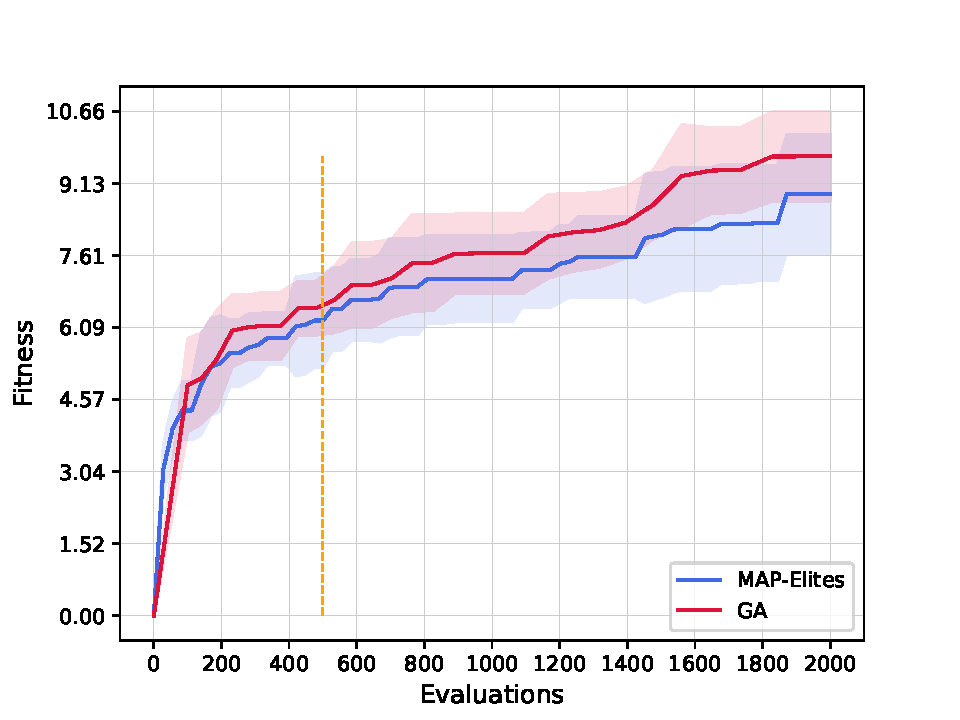
\includegraphics[scale=0.65]{images/body_opt/comp_qd_ga_w_ft}
    \caption{Walker task fitness trend comparison. The two algorithms reach high fitness values, and the two curves have similar shapes.}
    \label{fig:qd_ga_walker_ft}
\end{figure}

The performance grids in Figure \ref{fig:qd_ga_walker_pg} confirm that the two algorithms reach good fitness values, since they both have dark green coloured cells.\\
The main difference is that MAP-Elites widely fills the map, and the color is uniformly distributed, with a slightly brighter color in the center, whereas the GA map highlights that its best fitness values converge to a specific bin, and a noticeable color difference exists between that cell and the border ones.

\begin{figure}[h]
    \centering
    \begin{subfigure}[b]{0.49\textwidth}
         \centering
         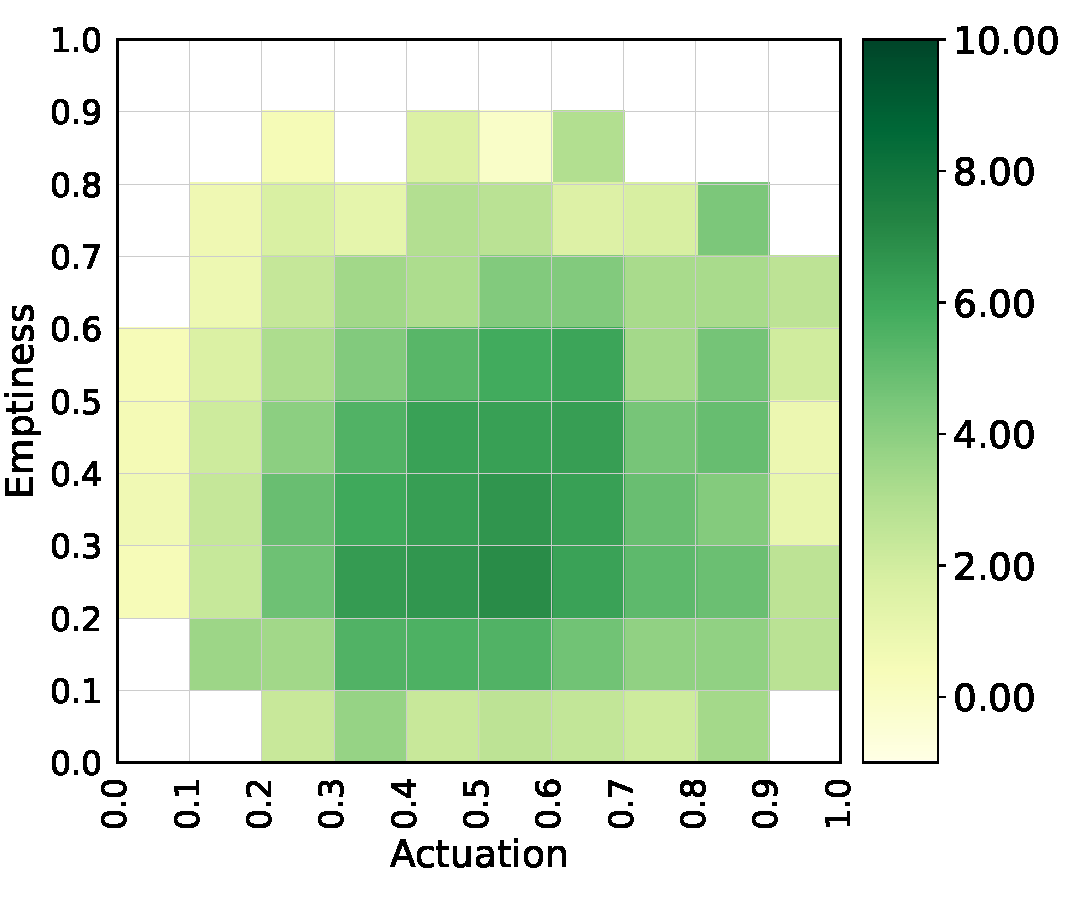
\includegraphics[scale=0.45]{images/body_opt/walker_qd_pg}
         \caption{MAP-Elites}
    \end{subfigure}
    \hfill
    \begin{subfigure}[b]{0.49\textwidth}
         \centering
         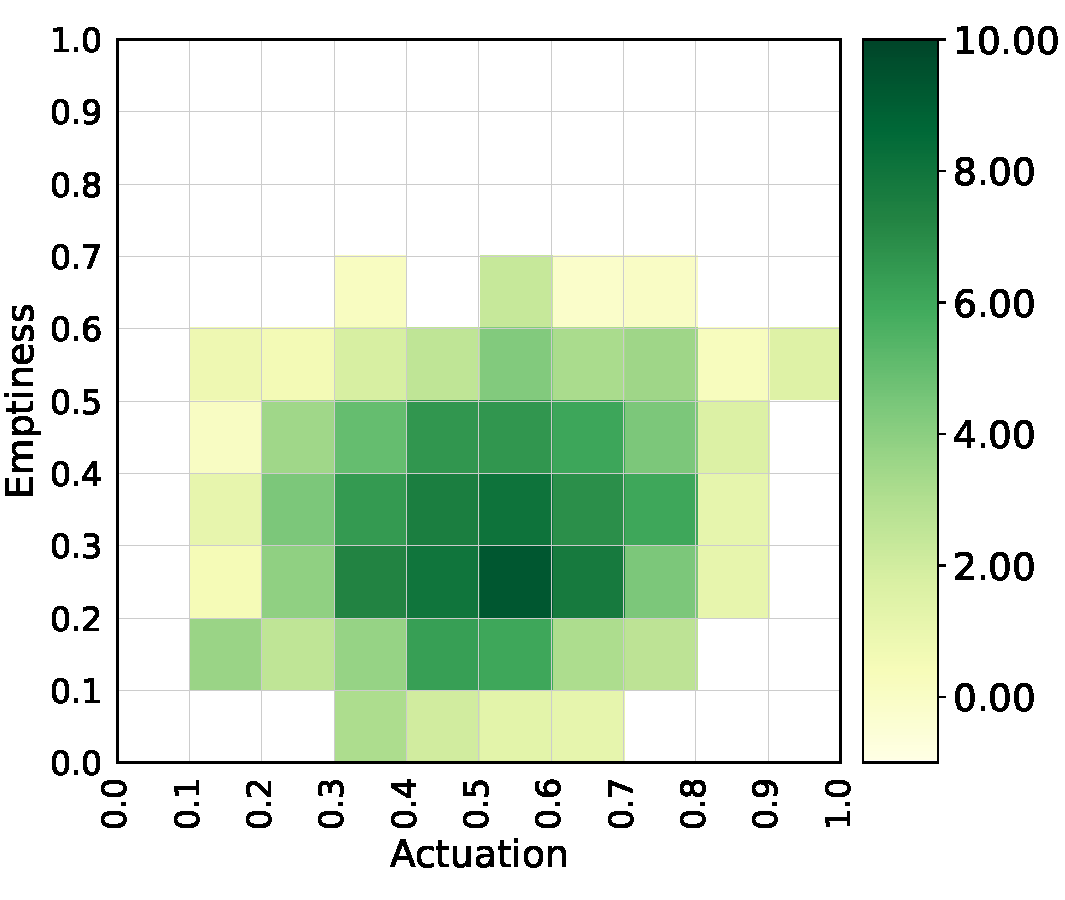
\includegraphics[scale=0.45]{images/body_opt/walker_ga_pg}
         \caption{GA}
    \end{subfigure}
    \caption{Walker task performance grid comparison. MAP-Elites (a) fills the map quite uniformly; GA (b) converges to a specific bin.}
    \label{fig:qd_ga_walker_pg}
\end{figure}

\subsection{Activity analysis}
An analysis on the activity maps, shown in Figure \ref{fig:qd_ga_walker_ag}, underlines the different approaches of the two design optimization algorithms.

The GA map shows that the value of a specific cell has been overwritten multiple times. It is not by chance that the most active cell is also the one with the best performance (in relation to Figure \ref{fig:qd_ga_walker_pg}): this is due to the fact the only goal of GA is to always get better performing individuals, selecting, and then mutating, the best ones at the end of each generation.

\begin{figure}[H]
    \centering
    \begin{subfigure}[b]{0.49\textwidth}
         \centering
         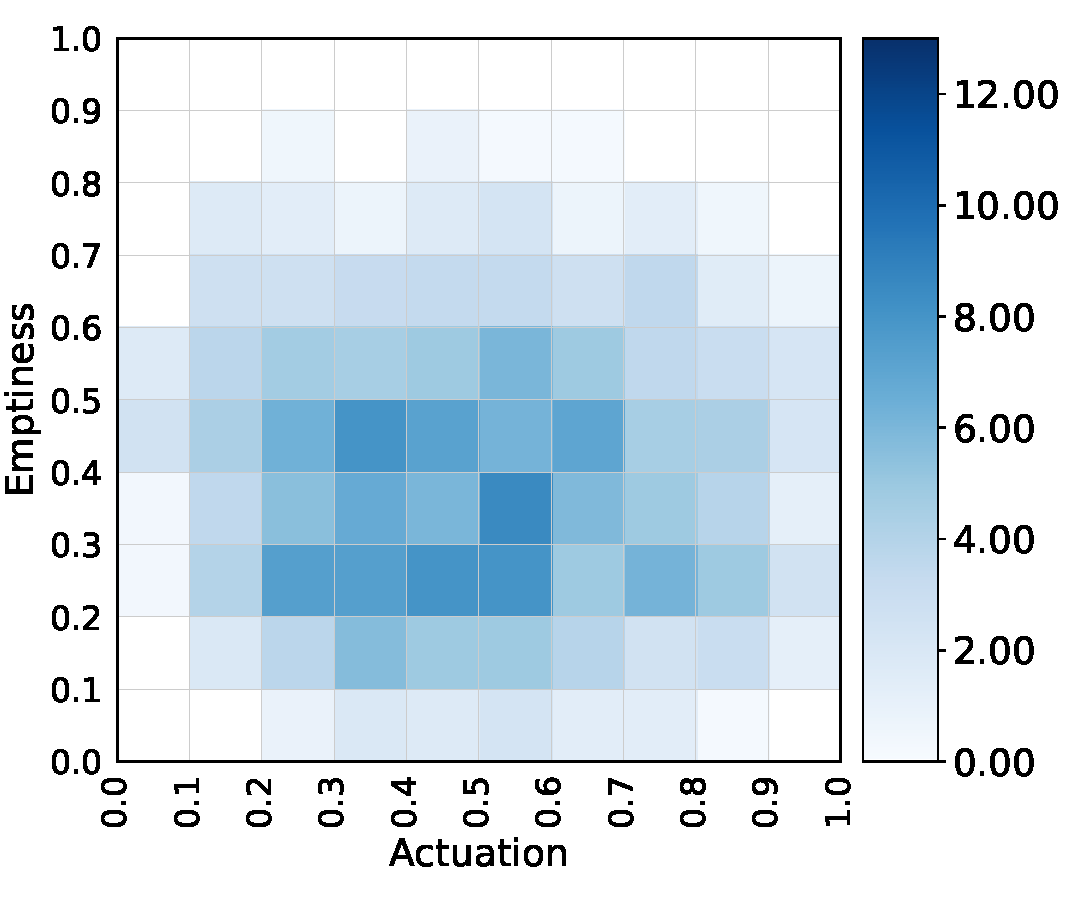
\includegraphics[scale=0.45]{images/body_opt/walker_qd_ag}
         \caption{MAP-Elites}
    \end{subfigure}
    \hfill
    \begin{subfigure}[b]{0.49\textwidth}
         \centering
         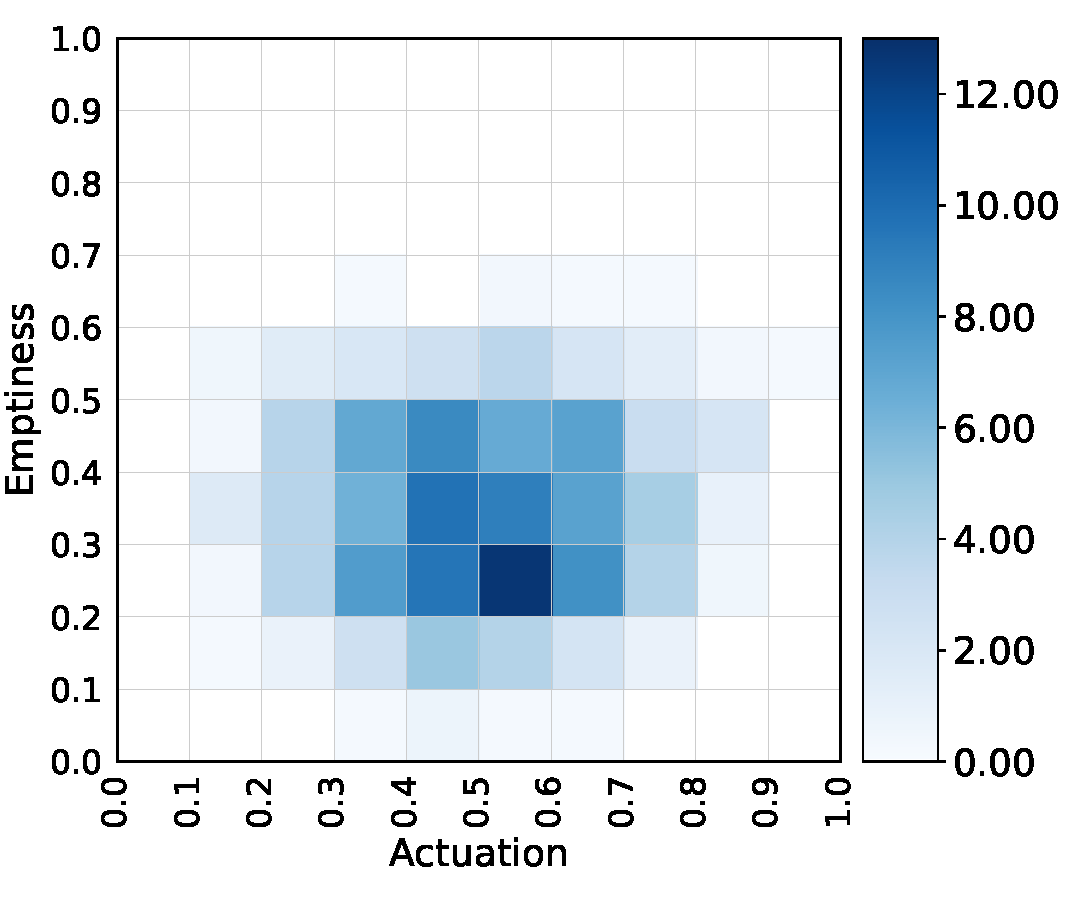
\includegraphics[scale=0.45]{images/body_opt/walker_ga_ag}
         \caption{GA}
    \end{subfigure}
    \caption{Walker task activity grid comparison. MAP-Elites (a) fills the map widely and uniformly; GA (b) focuses on few cells and converges to a specific bin, that coincides with the one with the best fitness value.}
    \label{fig:qd_ga_walker_ag}
\end{figure}

On the contrary, MAP-Elites activity map is uniform and it's not correlated to the performance map, confirming that the algorithm is not focused on the mere best fitness achievement. However, the cells in the center have a darker colour in comparison with the ones in the border. This is mainly because there's less chance of having individuals with feature values at the end of the domain.

Thanks to the activity trends in Figure \ref{fig:qd_ga_walker_at}, it is possible to analyze the number of explored bins in the map in relation to the number of evaluated individuals.\\
The curves of the two algorithms have similar shapes for the first 500 evaluations, which is the number of individuals that MAP-Elites generates randomly. After this threshold, the number of bins explored by MAP-Elites increases highly and quite constantly, whereas GA continues a much slower rise.
This confirms that promoting diversity also means promoting exploration of the feature domains.

\begin{figure}[h]
    \centering
    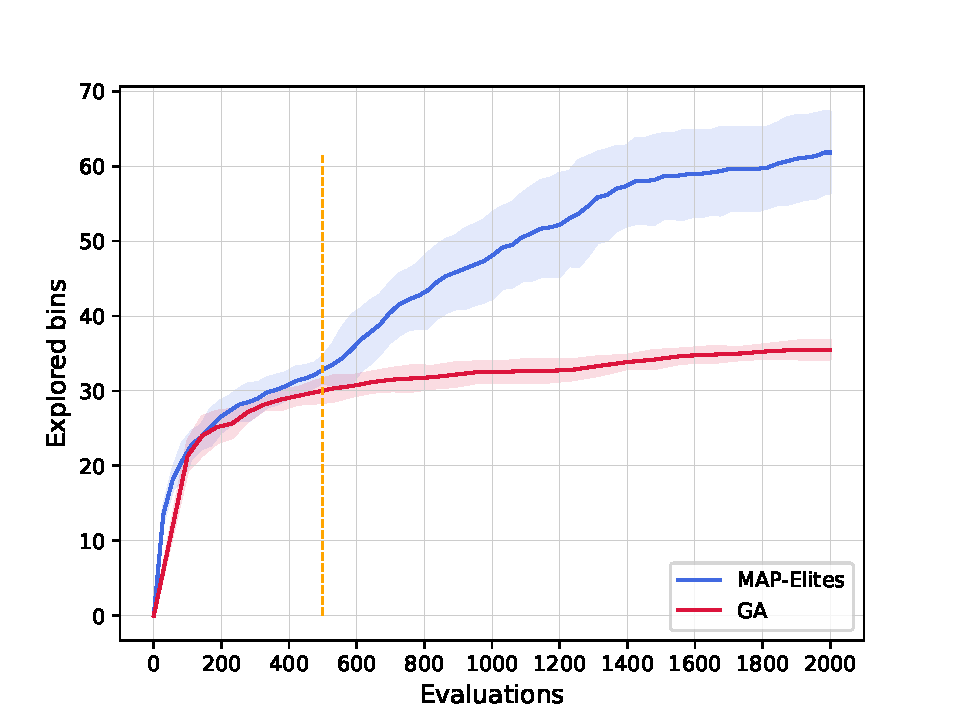
\includegraphics[scale=0.65]{images/body_opt/comp_qd_ga_w_at}
    \caption{Walker task activity trend comparison. After a generation of randomly generated bodies, MAP-Elites continuously explores different cells. GA, after the first few generations, has a much slower rise, since it focuses on few cells.}
    \label{fig:qd_ga_walker_at}
\end{figure}

\subsection{Top designs}
The morphologies of the best performing individuals emphasize the different approaches of the two algorithms.\\
Using GA, the best individuals per generation survive and new individuals can be generated by a mutation of those who survived. Therefore, the resulting top designs are very similar, as shown in Figure \ref{fig:ga_walker_topdesigns}.\\
MAP-Elites is a QD algorithm, therefore it promotes diversity: the best performing individuals, shown in Figure \ref{fig:qd_walker_topdesigns}, have different morphologies.\\
However, most of the top designs obtained by the two algorithms have a great number of horizontal actuators and they have grown two legs, which is what allows them to walk; this interesting result highlights once again the strong connection with biology, since they resemble natural creatures, even though they had no prior knowledge.

\begin{figure}[H]
    \centering
    \begin{tabular}{cccccc}
    \rule{0pt}{9ex}  
    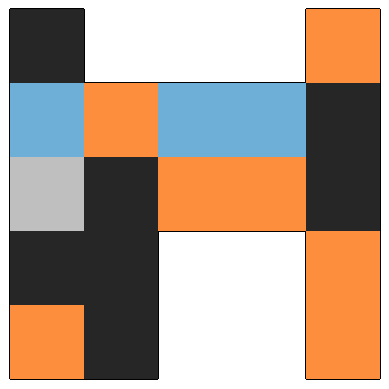
\includegraphics[scale=0.1]{images/top_designs/walker/ga/ga3_gen29_ind0} &
    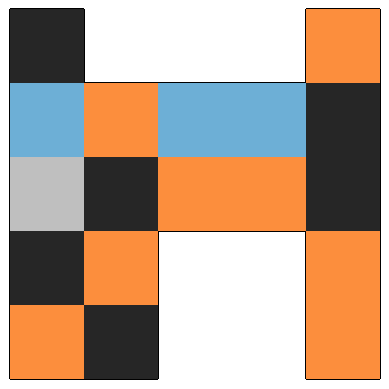
\includegraphics[scale=0.1]{images/top_designs/walker/ga/ga3_gen29_ind1} &
    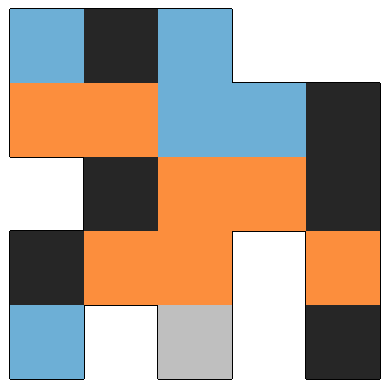
\includegraphics[scale=0.1]{images/top_designs/walker/ga/ga3_gen29_ind2} &
    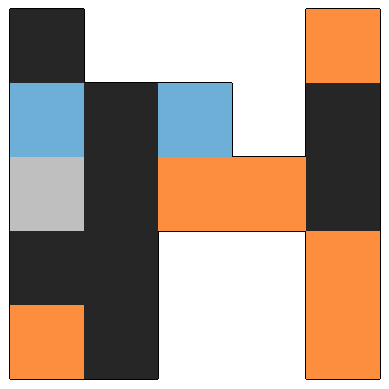
\includegraphics[scale=0.1]{images/top_designs/walker/ga/ga3_gen29_ind3} &
    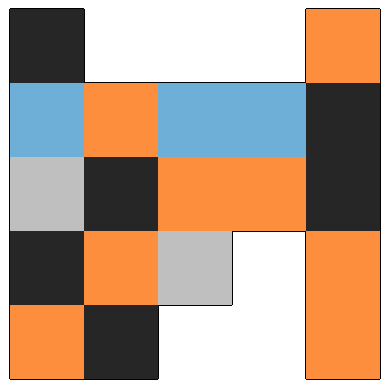
\includegraphics[scale=0.1]{images/top_designs/walker/ga/ga3_gen29_ind4} &
    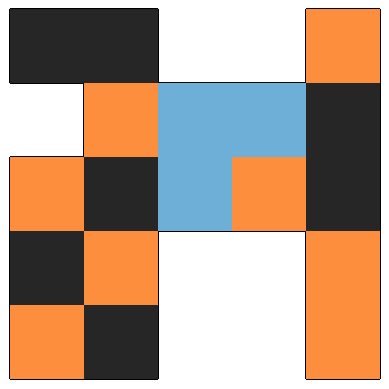
\includegraphics[scale=0.1]{images/top_designs/walker/ga/ga3_gen29_ind5} \\
    \hline \rule{0pt}{9ex}  
    
\includegraphics[scale=0.1]{images/top_designs/walker/ga/ga5_gen29_ind0} &
    
\includegraphics[scale=0.1]{images/top_designs/walker/ga/ga5_gen29_ind1} &
    
\includegraphics[scale=0.1]{images/top_designs/walker/ga/ga5_gen29_ind2} &
    
\includegraphics[scale=0.1]{images/top_designs/walker/ga/ga5_gen29_ind3} &
    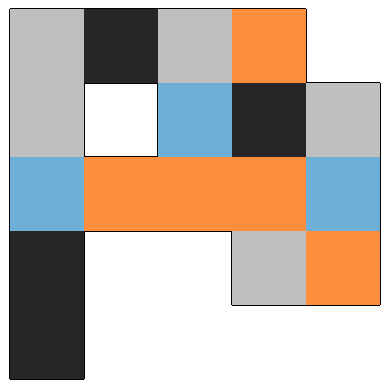
\includegraphics[scale=0.1]{images/top_designs/walker/ga/ga5_gen29_ind4} &
    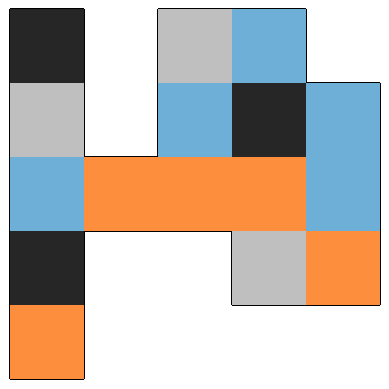
\includegraphics[scale=0.1]{images/top_designs/walker/ga/ga5_gen29_ind5}\\
    \hline \rule{0pt}{9ex}  
    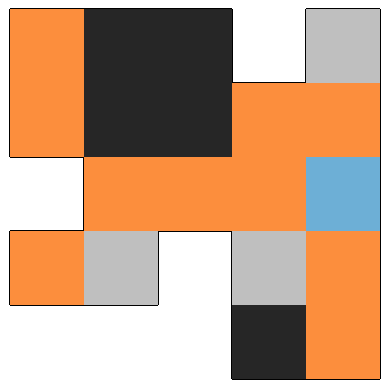
\includegraphics[scale=0.1]{images/top_designs/walker/ga/ga6_gen29_ind0} &
    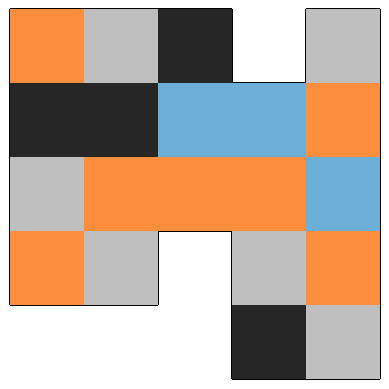
\includegraphics[scale=0.1]{images/top_designs/walker/ga/ga6_gen29_ind1} &
    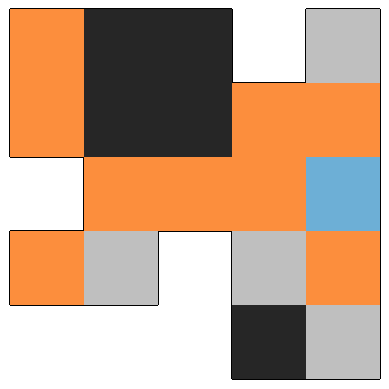
\includegraphics[scale=0.1]{images/top_designs/walker/ga/ga6_gen29_ind2} &
    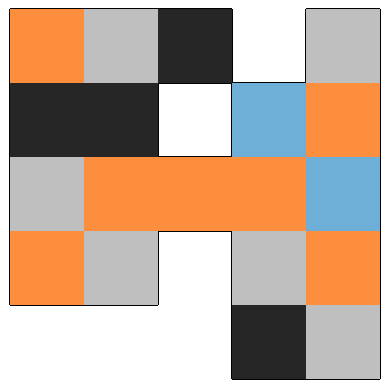
\includegraphics[scale=0.1]{images/top_designs/walker/ga/ga6_gen29_ind3} &
    
\includegraphics[scale=0.1]{images/top_designs/walker/ga/ga6_gen29_ind4} &
    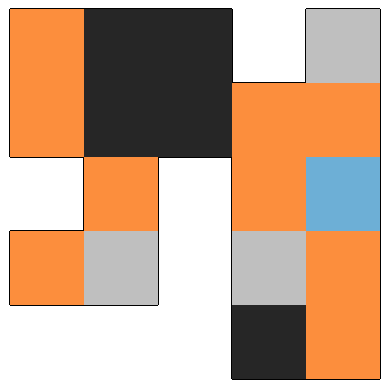
\includegraphics[scale=0.1]{images/top_designs/walker/ga/ga6_gen29_ind5}\\
\end{tabular}

    \caption{GA best performing morphologies on the walker task in three different experiments. For each experiment, top designs look very similar.}
    \label{fig:ga_walker_topdesigns}
\end{figure}

\begin{figure}[H]
    \centering
    \begin{tabular}{cccccc}
    \rule{0pt}{9ex}  
    
\includegraphics[scale=0.1]{images/top_designs/walker/map_elites/exp3/0_ind1668.png} &
    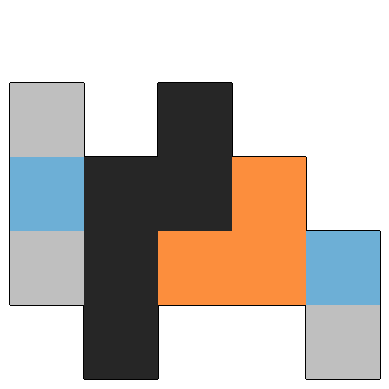
\includegraphics[scale=0.1]{images/top_designs/walker/map_elites/exp3/1_ind1839.png} &
    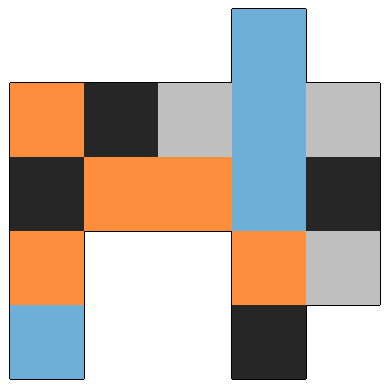
\includegraphics[scale=0.1]{images/top_designs/walker/map_elites/exp3/2_ind563.png} &
    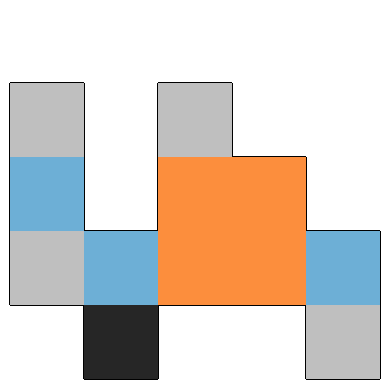
\includegraphics[scale=0.1]{images/top_designs/walker/map_elites/exp3/3_ind1860.png} &
    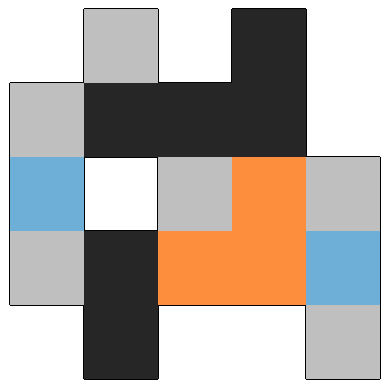
\includegraphics[scale=0.1]{images/top_designs/walker/map_elites/exp3/4_ind1297.png} &
    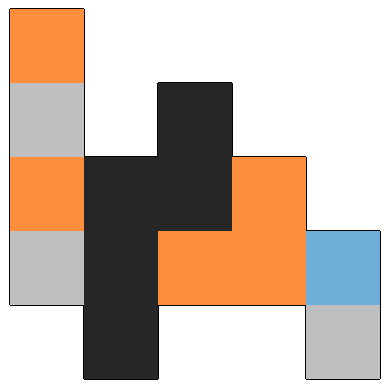
\includegraphics[scale=0.1]{images/top_designs/walker/map_elites/exp3/5_ind911.png}\\
    \hline \rule{0pt}{9ex}  
    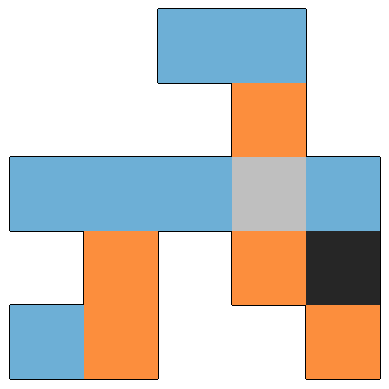
\includegraphics[scale=0.1]{images/top_designs/walker/map_elites/exp1/0_ind1650.png} &
    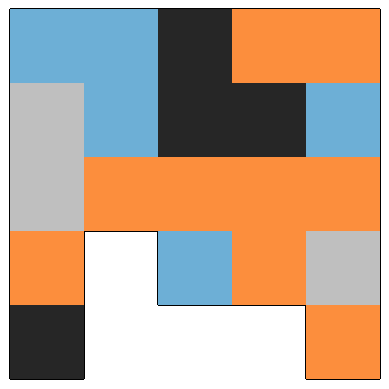
\includegraphics[scale=0.1]{images/top_designs/walker/map_elites/exp1/1_ind1719.png} &
    
\includegraphics[scale=0.1]{images/top_designs/walker/map_elites/exp1/2_ind1462.png} &
    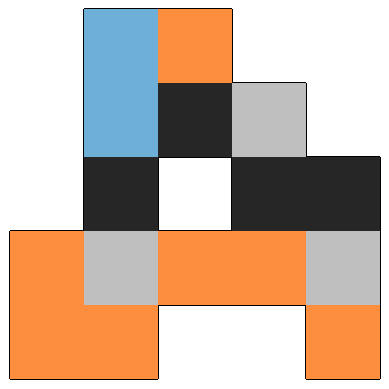
\includegraphics[scale=0.1]{images/top_designs/walker/map_elites/exp1/3_ind1481.png} &
    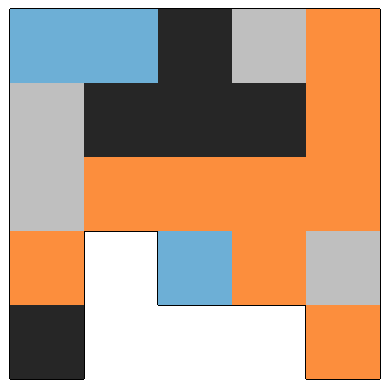
\includegraphics[scale=0.1]{images/top_designs/walker/map_elites/exp1/4_ind1559.png} &
    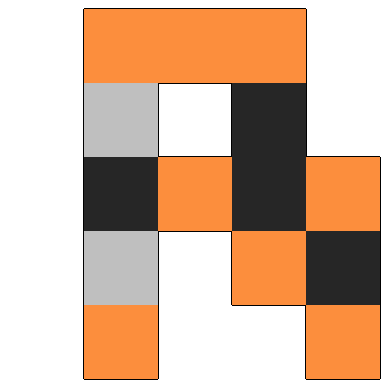
\includegraphics[scale=0.1]{images/top_designs/walker/map_elites/exp1/5_ind1270.png}\\
    \hline \rule{0pt}{9ex}  
    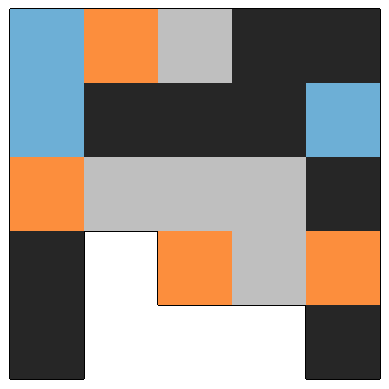
\includegraphics[scale=0.1]{images/top_designs/walker/map_elites/exp4/0_ind1535.png} &
    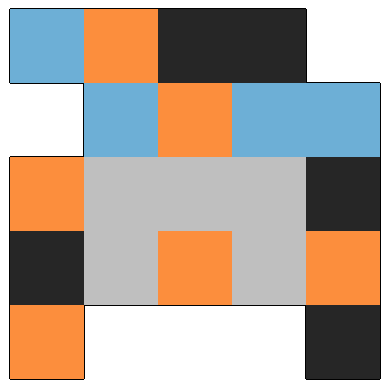
\includegraphics[scale=0.1]{images/top_designs/walker/map_elites/exp4/1_ind1775.png} &
    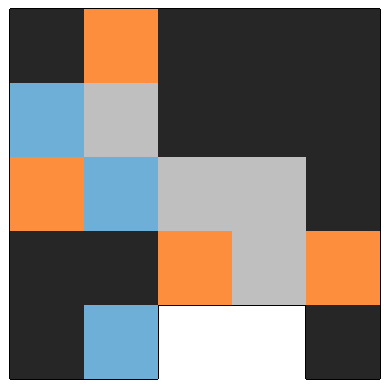
\includegraphics[scale=0.1]{images/top_designs/walker/map_elites/exp4/2_ind1692.png} &
    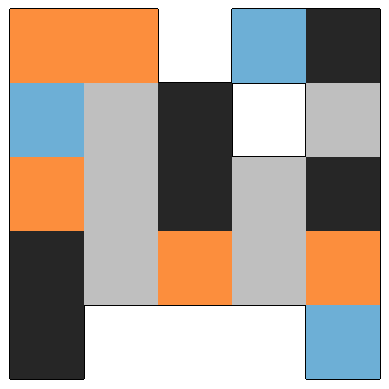
\includegraphics[scale=0.1]{images/top_designs/walker/map_elites/exp4/3_ind1759.png} &
    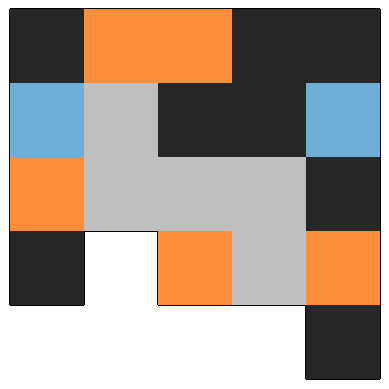
\includegraphics[scale=0.1]{images/top_designs/walker/map_elites/exp4/4_ind1183.png}&
    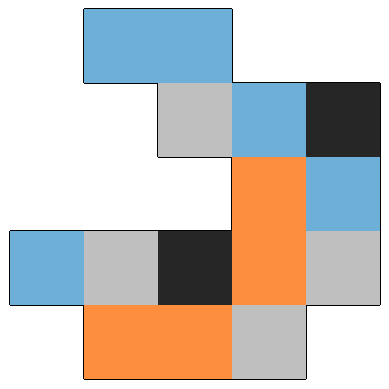
\includegraphics[scale=0.1]{images/top_designs/walker/map_elites/exp4/5_ind165.png}\\
\end{tabular}
    \caption{MAP-Elites best performing morphologies on the walker task in three different experiments. The algorithm produced well-performing individuals with various designs.}
    \label{fig:qd_walker_topdesigns}
\end{figure}


%%%%%%%%%%%%%%%%%%%%%%%% PUSHER %%%%%%%%%%%%%%%%%%%%%%%% 
\section{Pusher}
In this environment, the goal is to push an object as far as possible. To do so, individuals must also learn how to walk. The object can't be simply thrown, because a penalty is applied according to its distance from the body.

\subsection{Performance analysis}
An analysis on the performance map, in Figure \ref{fig:qd_ga_pusher_pg}, shows that GA finds well-performing individuals that are mapped on few close cells. On the contrary, MAP-Elites widely fills the map, and shows that even boundary cells, poorly touched by GA, can lead to interesting results.

The fitness trend comparison in Figure \ref{fig:qd_ga_pusher_ft} shows that the behaviour of the two algorithms in finding the best fitness value is very similar, especially for the first evaluations. This means that the two of them, after the same amount of evaluations, found vary similar, fitness values.\\
After further evaluations, they both continued their growth; the reduction of standard deviation in GA confirms that its behaviour is quite regular.

\begin{figure}[H]
    \centering
    \begin{subfigure}[b]{0.49\textwidth}
         \centering
         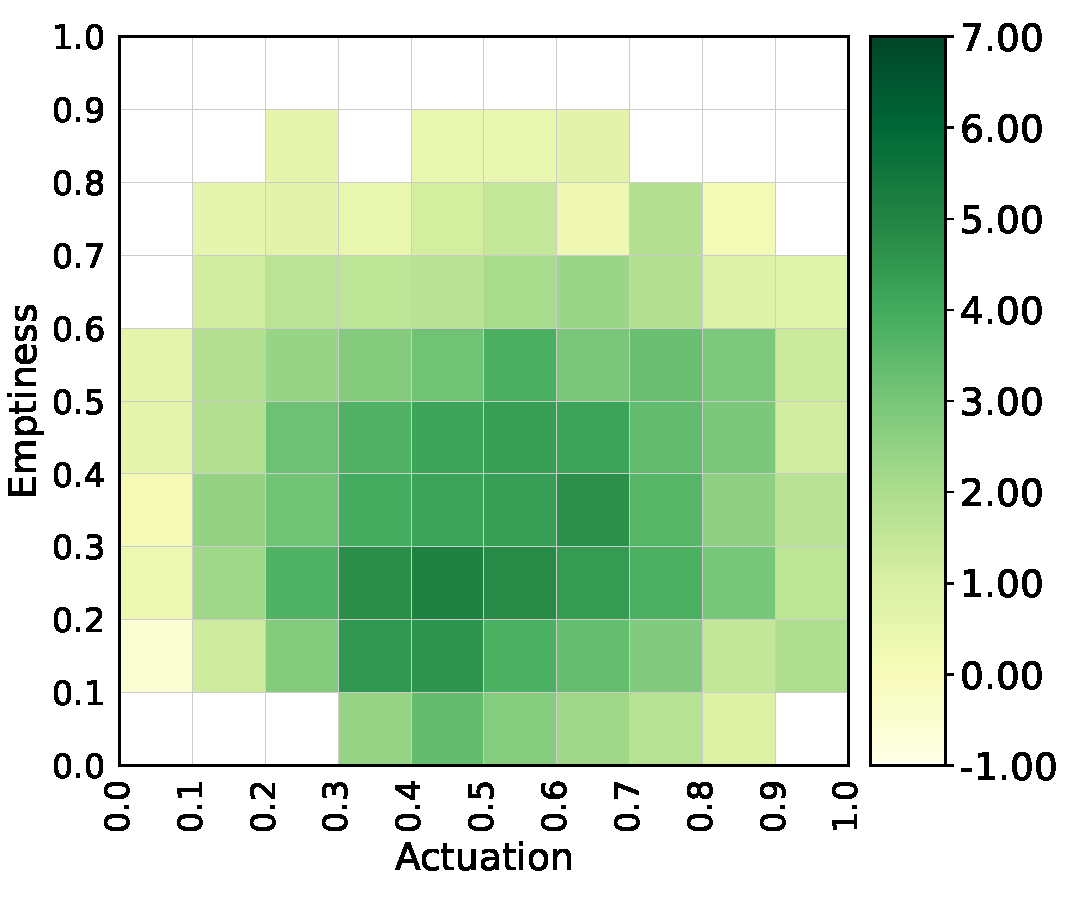
\includegraphics[scale=0.45]{images/brain_opt/pusher/pusher_qd_pg}
         \caption{MAP-Elites}
    \end{subfigure}
    \hfill
    \begin{subfigure}[b]{0.49\textwidth}
         \centering
         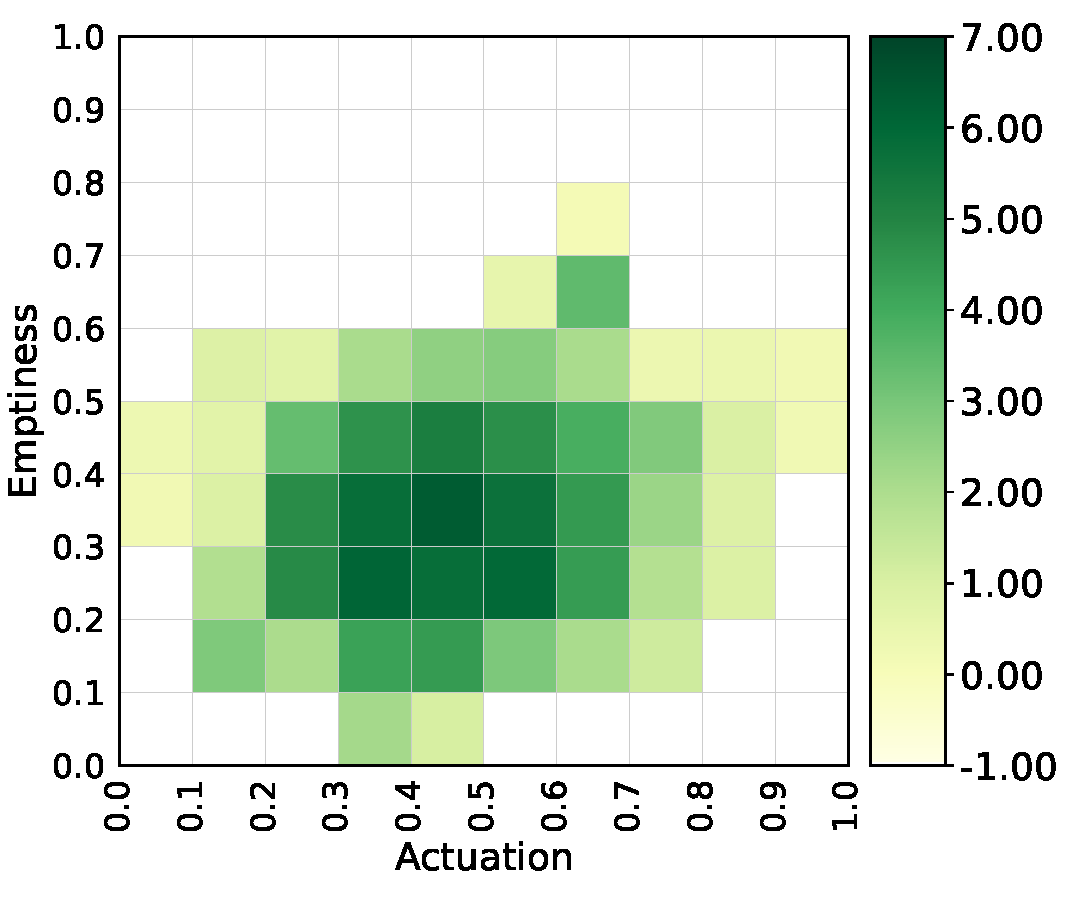
\includegraphics[scale=0.45]{images/brain_opt/pusher/pusher_ga_pg}
         \caption{GA}
    \end{subfigure}
    \caption{Pusher-v0 performance map comparison. GA (b) best performing individuals converge to few cells, while MAP-Elites map (a) is more uniform.}
    \label{fig:qd_ga_pusher_pg}
\end{figure}

\begin{figure}[H]
    \centering
    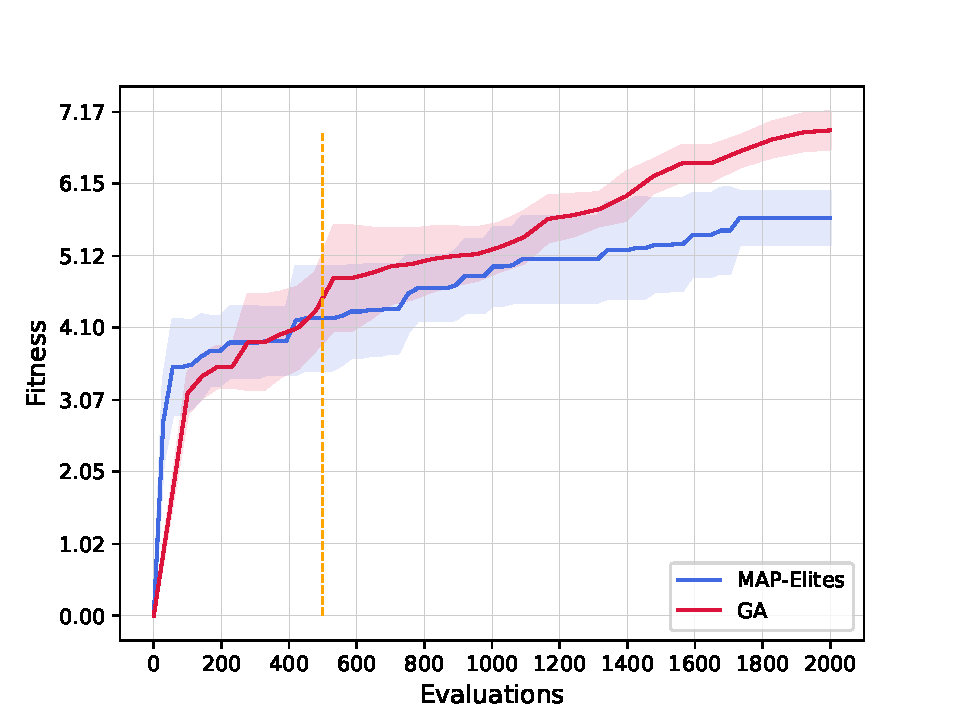
\includegraphics[scale=0.65]{images/brain_opt/pusher/comp_qd_ga_p_ft}
    \caption{Pusher-v0. Fitness trend comparison. The two algorithms have a similar behaviour, but GA gets higher fitness values.}
    \label{fig:qd_ga_pusher_ft}
\end{figure}

\subsection{Activity analysis}
As it was expected, the activity map of GA, shown in Figure \ref{fig:qd_ga_pusher_ag} focuses only on few cells. More specifically, border cells are the less visited, while it greatly focuses on the cells with the most common feature values. It's not by choice that the most overwritten cells are the one with the best fitness values.\\
On the contrary, MAP-Elites doesn't focus on few cells only. Its central area is more coloured, but there is not a small region that stands out. Also, its most overwritten cells do not coincide with the best performing ones, as it can be seen comparing the activity and the performance maps.

Comparing the number of explored bins behaviour, in Figure \ref{fig:qd_ga_pusher_at}, it is possible to distinguish two different moments. For the first 500 evaluations, the two lines almost coincide. The morphologies evaluated by MAP-Elites in this stage are randomly sampled, so it's an exploration stage. After further evaluations, GA continues a slow increase, that becomes steady at around 35\% of explored bins. On the contrary, MAP-Elites continues its rise to about 60\% of explored bins, almost twice as GA.\\
Also, the low standard deviation in the activity trend of GA confirms that this is a common behaviour for the algorithm, which focuses on the performance with no regards for the map exploration.

\begin{figure}[H]
    \centering
    \begin{subfigure}[b]{0.49\textwidth}
         \centering
         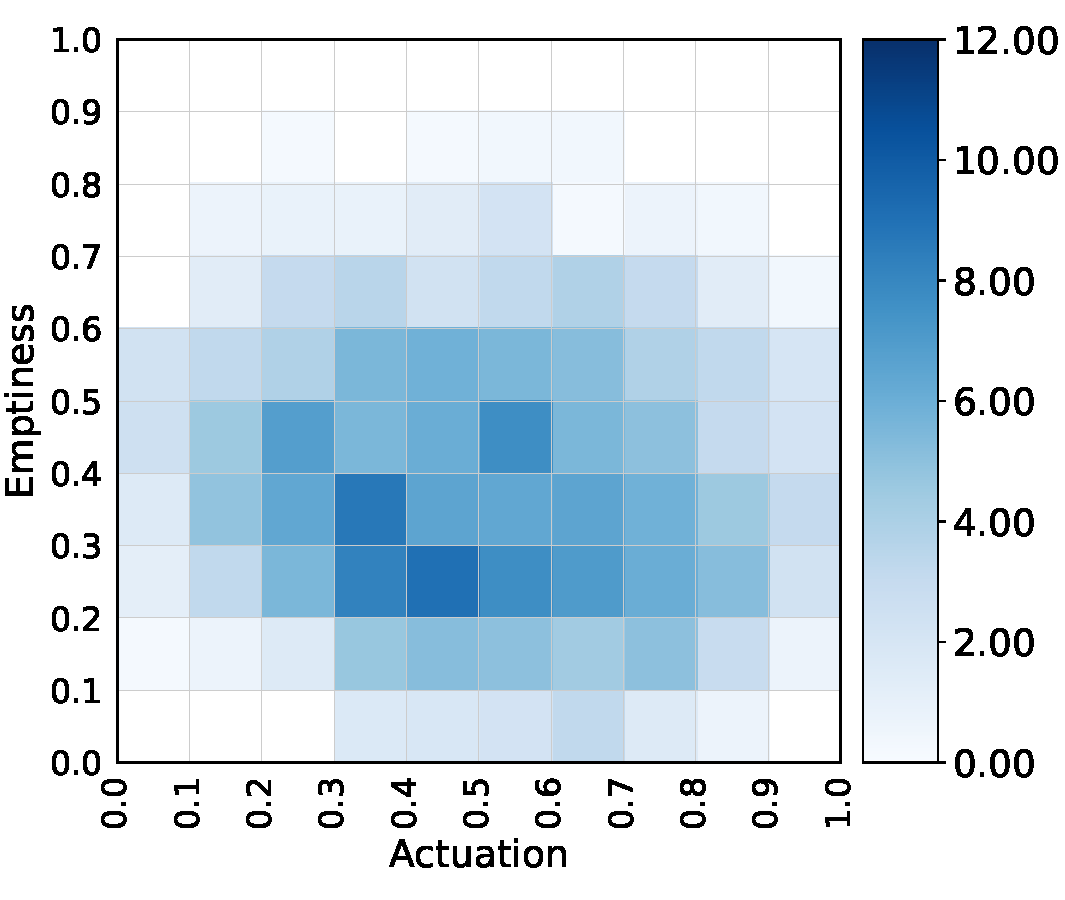
\includegraphics[scale=0.45]{images/brain_opt/pusher/pusher_qd_ag}
         \caption{MAP-Elites}
    \end{subfigure}
    \hfill
    \begin{subfigure}[b]{0.49\textwidth}
         \centering
         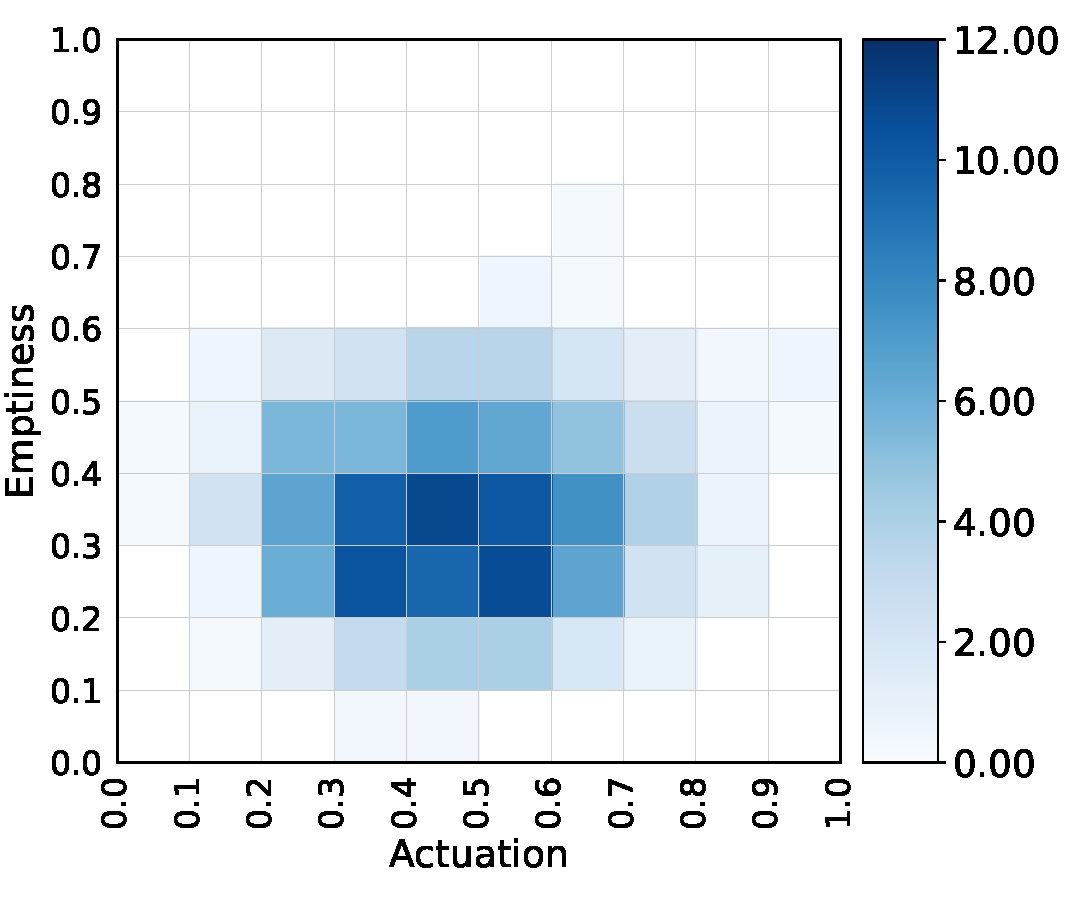
\includegraphics[scale=0.45]{images/brain_opt/pusher/pusher_ga_ag}
         \caption{GA}
    \end{subfigure}
    \caption{Pusher-v0 activity map comparison. GA (b) focuses on few cells only, while MAP-Elites map (a) is widely and more uniformely explored.}
    \label{fig:qd_ga_pusher_ag}
\end{figure}

\begin{figure}[H]
    \centering
    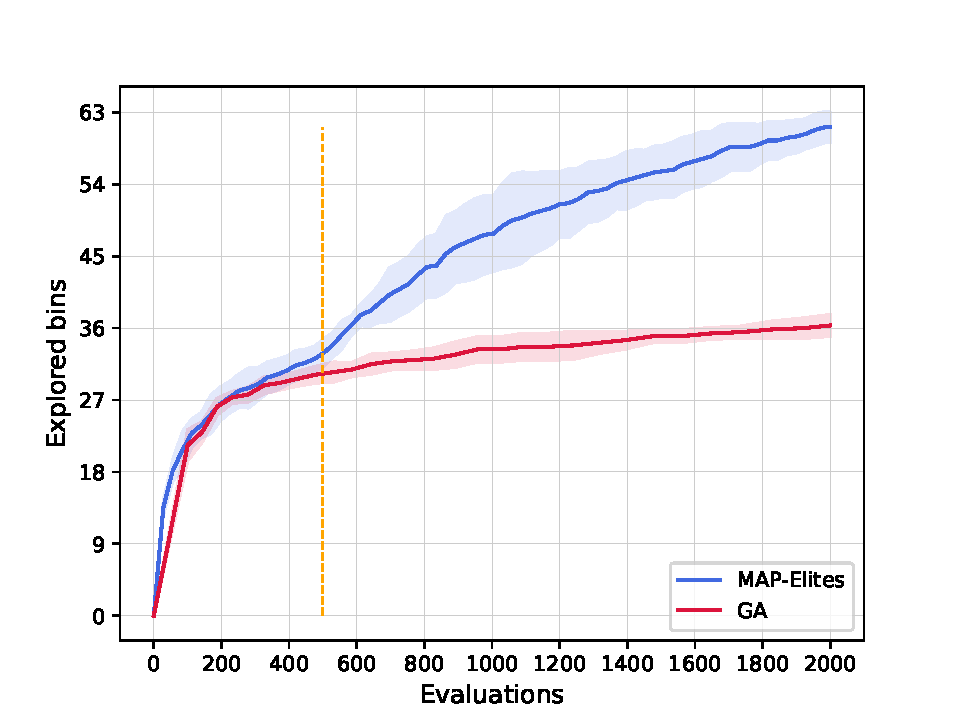
\includegraphics[scale=0.65]{images/brain_opt/pusher/comp_qd_ga_p_at}
    \caption{Pusher-v0. Activity trend comparison. After a generation of randomly generated bodies, MAP-Elites continuously explores different cells. GA, after the first few generations, has a much slower rise, since it focuses on few cells}
    \label{fig:qd_ga_pusher_at}
\end{figure}

\subsection{Top designs}
The designs of the best performing individuals behave differently according to the algorithm applied. The best individuals per generation found by GA are the ones to survive, and they can mutate to generate offspring. This is why the top designs look very similar, as shown in Figure \ref{fig:ga_pusher_topdesigns}. On the contrary, MAP-Elites promotes diversity, so the top designs obtained, in Figure \ref{fig:qd_pusher_topdesigns}, have different morphologies.
Since the pusher task also had the implicit goal of leaning to walk, most of the the individuals obtained grew legs.

\begin{figure}[H]
    \centering
    \begin{tabular}{cccccc}
    \rule{0pt}{9ex}  
    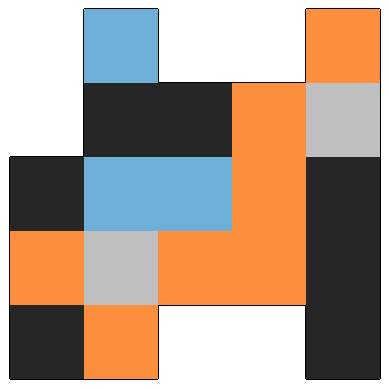
\includegraphics[scale=0.1]{images/top_designs/pusher/ga/exp1/gen29_ind0} &
    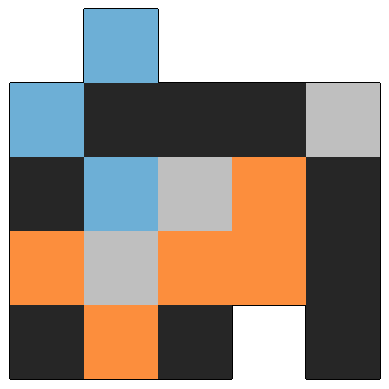
\includegraphics[scale=0.1]{images/top_designs/pusher/ga/exp1/gen29_ind1} &
    \includegraphics[scale=0.1]{images/top_designs/pusher/ga/exp1/gen29_ind2} &
    \includegraphics[scale=0.1]{images/top_designs/pusher/ga/exp1/gen29_ind3} &
    \includegraphics[scale=0.1]{images/top_designs/pusher/ga/exp1/gen29_ind4} &
    \includegraphics[scale=0.1]{images/top_designs/pusher/ga/exp1/gen29_ind5} \\
    \hline \rule{0pt}{9ex}  
    \includegraphics[scale=0.1]{images/top_designs/pusher/ga/exp3/gen29_ind0} &
    \includegraphics[scale=0.1]{images/top_designs/pusher/ga/exp3/gen29_ind1} &
    \includegraphics[scale=0.1]{images/top_designs/pusher/ga/exp3/gen29_ind2} &
    \includegraphics[scale=0.1]{images/top_designs/pusher/ga/exp3/gen29_ind3} &
    \includegraphics[scale=0.1]{images/top_designs/pusher/ga/exp3/gen29_ind4} &
    \includegraphics[scale=0.1]{images/top_designs/pusher/ga/exp3/gen29_ind5} \\
    \hline \rule{0pt}{9ex}  
    \includegraphics[scale=0.1]{images/top_designs/pusher/ga/exp5/gen29_ind0} &
    \includegraphics[scale=0.1]{images/top_designs/pusher/ga/exp5/gen29_ind1} &
    \includegraphics[scale=0.1]{images/top_designs/pusher/ga/exp5/gen29_ind2} &
    \includegraphics[scale=0.1]{images/top_designs/pusher/ga/exp5/gen29_ind3} &
    \includegraphics[scale=0.1]{images/top_designs/pusher/ga/exp5/gen29_ind4} &
    \includegraphics[scale=0.1]{images/top_designs/pusher/ga/exp5/gen29_ind5} \\
\end{tabular}

    \caption{GA best performing morphologies on the pusher task in three different experiments. For each experiment, top designs look very similar.}
    \label{fig:ga_pusher_topdesigns}
\end{figure}

\begin{figure}[H]
    \centering
    \begin{tabular}{cccccc}
    \rule{0pt}{9ex}  
    \includegraphics[scale=0.1]{images/top_designs/pusher/map_elites/exp6/0_ind1672.png} &
    \includegraphics[scale=0.1]{images/top_designs/pusher/map_elites/exp6/1_ind1573.png} &
    \includegraphics[scale=0.1]{images/top_designs/pusher/map_elites/exp6/2_ind1648.png} &
    \includegraphics[scale=0.1]{images/top_designs/pusher/map_elites/exp6/3_ind1796.png} &
    \includegraphics[scale=0.1]{images/top_designs/pusher/map_elites/exp6/4_ind1924.png} &
    \includegraphics[scale=0.1]{images/top_designs/pusher/map_elites/exp6/5_ind1516.png}\\
    \hline \rule{0pt}{9ex}  
    \includegraphics[scale=0.1]{images/top_designs/pusher/map_elites/exp4/0_ind1682.png} &
    \includegraphics[scale=0.1]{images/top_designs/pusher/map_elites/exp4/1_ind1334.png} &
    \includegraphics[scale=0.1]{images/top_designs/pusher/map_elites/exp4/2_ind1704.png} &
    \includegraphics[scale=0.1]{images/top_designs/pusher/map_elites/exp4/3_ind1961.png} &
    \includegraphics[scale=0.1]{images/top_designs/pusher/map_elites/exp4/4_ind1818.png} &
    \includegraphics[scale=0.1]{images/top_designs/pusher/map_elites/exp4/5_ind1698.png}\\
    \hline \rule{0pt}{9ex}  
    \includegraphics[scale=0.1]{images/top_designs/pusher/map_elites/exp2/0_ind1707.png} &
    \includegraphics[scale=0.1]{images/top_designs/pusher/map_elites/exp2/1_ind986.png} &
    \includegraphics[scale=0.1]{images/top_designs/pusher/map_elites/exp2/2_ind1731.png} &
    \includegraphics[scale=0.1]{images/top_designs/pusher/map_elites/exp2/3_ind1288.png} &
    \includegraphics[scale=0.1]{images/top_designs/pusher/map_elites/exp2/4_ind1057.png} &
    \includegraphics[scale=0.1]{images/top_designs/pusher/map_elites/exp2/5_ind1410.png}\\
\end{tabular}
    \caption{MAP-Elites best performing morphologies on the pusher task in three different experiments. The algorithm produced well-performing individuals with various designs.}
    \label{fig:qd_pusher_topdesigns}
\end{figure}


%%%%%%%%%%%%%%%%%%%%%%%% CARRIER %%%%%%%%%%%%%%%%%%%%%%%%
\section{Carrier}
In this task, the goal is to carry an object as far as possible.\\
The individuals trained in this task are supposed to learn how to walk and how to carry a box initialized in front of
them.

\subsection{Performance analysis}
A comparison of the performance grids in Figure \ref{fig:qd_ga_carrier_pg} show that MAP-Elites fills the map more widely than GA.\\
GA gets a higher best fitness value, and the distribution of color in its cells shows that the individuals with a good performance converge to few cells only. However, focusing on few cells only precludes it to find well-performing individuals in other map areas. On the contrary, MAP-Elites, exploring the map, found well performing individuals even on the boundary cells, never explored by GA.\\
Since a penalty is applied when the object falls under a certain height, some individuals stored in the map have a negative fitness value.

The fitness trend comparison in Figure \ref{fig:qd_ga_carrier_ft}, shows that GA has higher best-fitness values after all evaluation intervals. Even though they sometimes get very close, MAP-Elites never obtains a higher best-fitness value. This is mainly because GA focuses on obtaining the best individual, therefore it selects its best performing robots to survive and, potentially, mutate. On the contrary, the selection of individuals to mutate in MAP-Elites is not driven by their fitness value.

\begin{figure}[H]
    \centering
    \includegraphics[scale=0.65]{images/brain_opt/carrier/comp_qd_ga_c_ft}
    \caption{Carrier-v0. Fitness trend comparison.
    The two algorithms have a similar behaviour, but GA gets higher fitness values.}
    \label{fig:qd_ga_carrier_ft}
\end{figure}

\begin{figure}[H]
    \centering
    \begin{subfigure}[b]{0.49\textwidth}
         \centering
        \includegraphics[scale=0.45]{images/brain_opt/carrier/carrier_qd_pg}
         \caption{MAP-Elites}
    \end{subfigure}
    \hfill
    \begin{subfigure}[b]{0.49\textwidth}
         \centering
         \includegraphics[scale=0.45]{images/brain_opt/carrier/carrier_ga_pg}
         \caption{GA}
    \end{subfigure}
    \caption{Carrier-v0 performance map comparison. GA (b) best performing individuals converge to few cells, while MAP-Elites map (a) is more uniform.}
    \label{fig:qd_ga_carrier_pg}
\end{figure}

\subsection{Activity analysis}
The activity trend comparison in Figure \ref{fig:qd_ga_carrier_at} highlights the different approaches the two algorithms have in exploring the map.\\
GA has a rapid growth in the first evaluations, but then it remains stable at around 35\% of explored bins.
On the contrary, MAP-Elites has a gradual rise for all the experiment, leading to an almost doubled number of explored cells, compared to GA.

\begin{figure}[h]
    \centering
    \includegraphics[scale=0.65]{images/brain_opt/carrier/comp_qd_ga_c_at}
    \caption{Carrier-v0. Activity trend comparison.
    After a generation of randomly generated bodies, MAP-Elites continuously explores different cells. GA, after the first few generations, has a much slower rise, since it focuses on few cells}
    \label{fig:qd_ga_carrier_at}
\end{figure}

This is mainly because GA tends to focus on few cells, as illustrated in Figure \ref{fig:qd_ga_carrier_ag}, and trying to get better fitness values from individuals with the same features becomes always harder.\\
The activity map of MAP-Elites is widely filled, and picking from the many cells with lower fitness values, as previously analyzed from Figure \ref{fig:qd_ga_carrier_pg}, increases the chance to overwrite them.

\begin{figure}[H]
    \centering
    \begin{subfigure}[b]{0.49\textwidth}
         \centering
         \includegraphics[scale=0.45]{images/brain_opt/carrier/carrier_qd_ag}
         \caption{MAP-Elites}
    \end{subfigure}
    \hfill
    \begin{subfigure}[b]{0.49\textwidth}
         \centering
         \includegraphics[scale=0.45]{images/brain_opt/carrier/carrier_ga_ag}
         \caption{GA}
    \end{subfigure}
    \caption{Carrier-v0 activity map comparison. GA (b) focuses on few cells only, while MAP-Elites map (a) is widely and more uniformely explored.}
    \label{fig:qd_ga_carrier_ag}
\end{figure}

\subsection{Top designs}
GA and MAP-Elites are designed with different goals: the first focuses on obtaining the best performance, the last one on the diversity. This difference is reflected on the resulting top designs. While individuals found by GA, Figure \ref{fig:ga_carrier_topdesigns} look evidently very similar, the ones obtained by MAP-Elites, shown in Figure \ref{fig:qd_carrier_topdesigns}, don't.
However, the two algorithms agree on the need of extra space above the individual to carry the box. Even though it was not a constraint of the task, all the best performing carriers have empty voxels above them, surrounded by few non-empty voxels to keep them from falling forward or backwards.

\begin{figure}[H]
    \centering
    \begin{tabular}{cccccc}
    \rule{0pt}{9ex}  
    \includegraphics[scale=0.1]{images/top_designs/carrier/ga/exp1/gen29_ind0} &
    \includegraphics[scale=0.1]{images/top_designs/carrier/ga/exp1/gen29_ind1} &
    \includegraphics[scale=0.1]{images/top_designs/carrier/ga/exp1/gen29_ind2} &
    \includegraphics[scale=0.1]{images/top_designs/carrier/ga/exp1/gen29_ind3} &
    \includegraphics[scale=0.1]{images/top_designs/carrier/ga/exp1/gen29_ind4} &
    \includegraphics[scale=0.1]{images/top_designs/carrier/ga/exp1/gen29_ind5} \\
    \hline \rule{0pt}{9ex}  
    \includegraphics[scale=0.1]{images/top_designs/carrier/ga/exp2/gen29_ind0} &
    \includegraphics[scale=0.1]{images/top_designs/carrier/ga/exp2/gen29_ind1} &
    \includegraphics[scale=0.1]{images/top_designs/carrier/ga/exp2/gen29_ind2} &
    \includegraphics[scale=0.1]{images/top_designs/carrier/ga/exp2/gen29_ind3} &
    \includegraphics[scale=0.1]{images/top_designs/carrier/ga/exp2/gen29_ind4} &
    \includegraphics[scale=0.1]{images/top_designs/carrier/ga/exp2/gen29_ind5} \\
    \hline \rule{0pt}{9ex}  
    \includegraphics[scale=0.1]{images/top_designs/carrier/ga/exp5/gen29_ind0} &
    \includegraphics[scale=0.1]{images/top_designs/carrier/ga/exp5/gen29_ind1} &
    \includegraphics[scale=0.1]{images/top_designs/carrier/ga/exp5/gen29_ind2} &
    \includegraphics[scale=0.1]{images/top_designs/carrier/ga/exp5/gen29_ind3} &
    \includegraphics[scale=0.1]{images/top_designs/carrier/ga/exp5/gen29_ind4} &
    \includegraphics[scale=0.1]{images/top_designs/carrier/ga/exp5/gen29_ind5} \\
\end{tabular}

    \caption{GA best performing morphologies on the carrier task in three different experiments. For each experiment, top designs look very similar.}
    \label{fig:ga_carrier_topdesigns}
\end{figure}

\begin{figure}[H]
    \centering
    \begin{tabular}{cccccc}
    \rule{0pt}{9ex}  
    \includegraphics[scale=0.1]{images/top_designs/carrier/map_elites/exp5/0_ind1365.png} &
    \includegraphics[scale=0.1]{images/top_designs/carrier/map_elites/exp5/1_ind1454.png} &
    \includegraphics[scale=0.1]{images/top_designs/carrier/map_elites/exp5/2_ind1424.png} &
    \includegraphics[scale=0.1]{images/top_designs/carrier/map_elites/exp5/3_ind1916.png} &
    \includegraphics[scale=0.1]{images/top_designs/carrier/map_elites/exp5/4_ind1631.png} &
    \includegraphics[scale=0.1]{images/top_designs/carrier/map_elites/exp5/5_ind1981.png}\\
    \hline \rule{0pt}{9ex}  
    \includegraphics[scale=0.1]{images/top_designs/carrier/map_elites/exp1/0_ind1505.png} &
    \includegraphics[scale=0.1]{images/top_designs/carrier/map_elites/exp1/1_ind869.png} &
    \includegraphics[scale=0.1]{images/top_designs/carrier/map_elites/exp1/2_ind1867.png} &
    \includegraphics[scale=0.1]{images/top_designs/carrier/map_elites/exp1/3_ind1113.png} &
    \includegraphics[scale=0.1]{images/top_designs/carrier/map_elites/exp1/4_ind1744.png} &
    \includegraphics[scale=0.1]{images/top_designs/carrier/map_elites/exp1/5_ind937.png}\\
    \hline \rule{0pt}{9ex}  
    \includegraphics[scale=0.1]{images/top_designs/carrier/map_elites/exp3/0_ind1737.png} &
    \includegraphics[scale=0.1]{images/top_designs/carrier/map_elites/exp3/1_ind712.png} &
    \includegraphics[scale=0.1]{images/top_designs/carrier/map_elites/exp3/2_ind862.png} &
    \includegraphics[scale=0.1]{images/top_designs/carrier/map_elites/exp3/3_ind1541.png} &
    \includegraphics[scale=0.1]{images/top_designs/carrier/map_elites/exp3/4_ind984.png} &
    \includegraphics[scale=0.1]{images/top_designs/carrier/map_elites/exp3/5_ind205.png}\\
\end{tabular}
    \caption{MAP-Elites best performing morphologies on the carrier task in three different experiments. The algorithm produced well-performing individuals with various designs.}
    \label{fig:qd_carrier_topdesigns}
\end{figure}



\section{Conclusion}
The Genetic Algorithm finds greater fitness values but, after a short initial exploration of the map, it focuses only on few cells. The most explored bins correspond to the ones with the greatest fitness, and this is because the fittest individuals survive through generations, therefore they are more likely to be selected and mutated, to generate new individuals.
As a consequence, the top individuals have very similar designs.\\
On the contrary, MAP-Elites widely explores the map and evaluates individuals with different feature values. Even though the central area in the map is usually the most visited, due to the higher chance of having bodies with medium feature values, boundary cells are not disregarded, and they can lead to interesting results. 
Since this algorithm promotes diversity, the individuals with the best fitness have various morphologies.\\
Even though the best fitness found by MAP-Elites algorithm is always lower than the one reached by GA, it does not disappoint. This results confirm that QD algorithms can find well performing individuals, that might be rejected by other reward-oriented algorithms like GA.\\
However, the two algorithms evolved robot bodies with some similarities: they grew legs or evolved space to carry an object, according to their task goal, resembling natural creatures even with no prior knowledge.


\newpage